\section{APLICAÇÕES DA TRI}
	\subsection{Introdução}
	\paragraph{}
	     A TRI, por se tratar de uma teoria de traço latente é aplicada a campos como a psicologia nos diagnósticos cognitivos e psicológicos. Também pode ser utilizada em várias outra situações onde busca-se medição de características ocultas, como no trabalho de \textcite{JessicaMaria} que usa o modelo de Rasch para avaliar o inventário de ansiedade de uma determinada escola, mostrando que características psicológicas como ansiedade podem interferir no desempenho dos alunos, assim surge a importância do diagnóstico precoce e correto da ansiedade na escola, por meio da identificação das dificuldades escolares apresentadas pelos alunos que vem crescendo na atualidade. Neste contexto, novas concepções sobre o processo de ensino e aprendizagem vêm reforçando a importância da influência das variáveis internas como as escolhas, crenças, expectativas e emoções, tanto daqueles que ensinam como daqueles que aprendem, os modelos que incluem ansiedade e outros fatores emocionais são modelos logísticos de 4 parâmetros, no qual este quarto parâmetro é adicionado. As aplicações da Teoria de Resposta ao Item são amplamente utilizadas em avaliações educacionais, devido ao crescimento e popularização do Enem, o objetivo deste trabalho é mostrar a TRI no aspecto da estimação da habilidade destes alunos.
	\par
    	Segundo \textcite{MOREIRAJUNIOR}, devido ao aumento do número de publicações: teses, dissertações, monografias, apresentações em congressos e publicações em periódicos, principalmente a partir do início do século XXI. A tendência é que a Teoria de Resposta ao Item seja aplicada cada vez mais nas mais diversas áreas.
    \par
    	No Brasil, a primeira obra exclusivamente sobre a TRI foi o livro "Teoria da Resposta ao Item: Conceitos e Aplicações”\cite{Dalton}, dos professores Dalton Francisco de Andrade, do Instituto de Informática e Estatística da UFSC, e Heliton Ribeiro Tavares, do Departamento de Estatística da UFPA, e da estatista da Fundação Carlos Chagas (FCC), Raquel da Cunha Valle.
    \par
    	Segundo JR (2010), a Teoria de Resposta ao Item passou a ser utilizada no Brasil em avaliação em grande escala com o ENEM em 2009. Porém, já vinha sendo utilizada desde 1995, Quando criado em 1998 o ENEM utilizava a TCT para cálculo das notas dos estudantes, mas a partir de 2009 o ENEM , que faz parte do sistema de avaliação responsáveis por aferir a qualidade da educação básica dos estudantes do ensino médio no Brasil,começa a utilizar a TRI para obtenção das notas destes estudantes. sendo o ENEM uma das principais aplicações da TRI e uma das maiores do Brasil visto o número de participantes que fizeram inscrição nos anos.
    \begin{figure}[!h]
		\centering
		\caption{Histórico de inscrições de 2009 a 2017}
		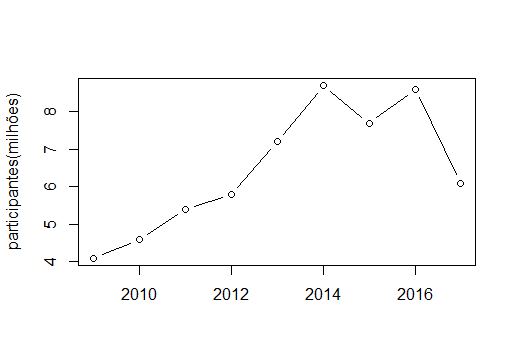
\includegraphics[width=0.5\linewidth]{img/parci}\\
		fonte: INEP(2017)
		\label{fig:parci}
	\end{figure}
    \paragraph{}
    	Entretanto existem críticas a este sistema, Segundo Barretto(2001) os sistemas de avaliação utilizam metodologias e procedimentos altamente sofisticados e se apoiam em um referencial diferente do que habitualmente utilizam os professores, o que pode contribuir para imprimir resistências nas escolas quanto à utilização dos resultados das avaliações.
    	%http://www.ufjf.br/ppge/files/2010/07/Disserta%C3%A7%C3%A3o-flavia-perry.pdf
    \subsection{Enem}
    \paragraph{}
    	De acordo com o MEC para a elaboração  de uma prova  tem-se a necessidade do conhecimento dos parâmetros dos itens. Sendo obtido através de pré-testagens de itens em amostras apropriadas de alunos nas quais estimamos os parâmetros dos itens em uma mesma escala de proficiência. Dessa maneira coloca-se os itens em uma escala de acordo com o nível de proficiência que eles exigem. O conjunto desses itens passa a formam o banco de itens na escala de proficiência desejada e a partir dele pode-se construir um ou mais testes com graus de dificuldade apropriados para atender os objetivos de uma ou mais avaliações. O importante é que as proficiências de alunos submetidos a esses diferentes testes são medidas na mesma escala e, portanto, comparáveis entre si. Da mesma forma, as medidas que se obtêm da proficiência de um aluno submetido a dois testes construídos com itens desse banco serão iguais.
	    O MEC descreve desta forma a pré-testagem, elaboração de itens.
	\subsubsection{Elaboração dos itens}
	\paragraph{}
    	Para que os itens sejam elaborados o Inep recorre a parcerias com instituições de educação superior interessadas em elaborar e revisar itens para a composição das provas do Enem. Estas parcerias têm o objetivo de aumentar a participação da comunidade acadêmica de todo o Brasil nos processos de avaliação educacional, agregando experiência, conhecimento e diversidade.
    \subsubsection{Banco Nacional de itens (BNI)}
    	\paragraph{}
    	Há a necessidade da criação de uma quantidade enorme de itens sendo o Enem é uma avaliação de larga escala, para isso aconteça o INEP gerencia o BNI que consiste em um banco de dados no qual os itens de provas são armazenados de forma segura. Esses itens ficam disponíveis para a construção de provas. A manutenção do BNI depende da entrada constante de itens de qualidade.
    \subsubsection{Pré-teste}
    \paragraph{}
    	Este é processo fundamental da calibração dos itens, que consiste na aplicação de um teste contendo itens a uma amostra de alunos com características semelhantes às da população para a qual a prova se destina. É a forma empírica de se avaliar a qualidade técnico-pedagógica e psicométrica dos itens. Essa etapa tem como objetivo captar subsídios importantes para aumentar a precisão da prova que será aplicada a milhões de participantes do Enem.
    \subsubsection{Análise depois do Pré-teste}
    \paragraph{}
	    A partir das respostas dos alunos, realiza-se uma série de análises estatísticas e pedagógicas; por exemplo, avaliam-se a dificuldade do item, a capacidade de discriminação e a possibilidade de acerto ao acaso. Depois dessas análises, as questões que atendem aos critérios ficam disponíveis para a montagem das provas, e as demais questões são descartadas ou encaminhadas para reformulação. o enem utilizam o método denominado Expected a Posteriori (EAP).\\
	    \textbf{Questão adequada} - Encaminhada ao Banco Nacional de Itens e utilizada para a elaboração das provas.\\
	    \textbf{Questão inadequada} - Retorna para reformulação ou descarte.\\
	\subsubsection{Elaboração das provas}
	\paragraph{}
    	Durante a seleção dos itens para a composição de uma prova, os índices psicométricos obtidos a partir do pré-teste são utilizados. Outras características consideradas são: conteúdo abordado, temática e habilidade da matriz de referência.
	\begin{figure}[!h]
		\centering
		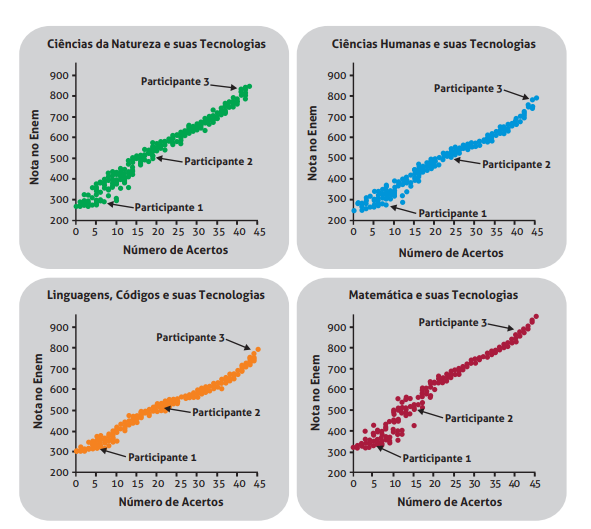
\includegraphics[width=0.4\linewidth]{img/acero}
		\caption{}
		\label{fig:acero}
	\end{figure}
	\paragraph{}
    	Observe que se a nota da TRI fosse exatamente o número de acertos, os pontos nos gráficos estariam alinhados representando uma reta. As variações desses pontos em relação à reta mostram que participantes com o mesmo número de acertos podem ter notas diferentes no Enem. Note, no entanto, que essa variação não é tão grande. O que nos leva a pergunta: Então por que o MEC utiliza a TRI? A resposta está na nota técnica publicada em 2012, onde o MEC diz que: A decisão de implementar no Exame Nacional do Ensino Médio (ENEM) a Teoria de Resposta ao Item (TRI) teve duas finalidades principais:
    \begin{enumerate}
        \item[(1)] permitir a comparabilidade dos resultados entre os anos.
        \item[(2)] permitir a aplicação do Exame várias vezes ao ano. Candidatos poderiam alegar que diferentes provas poderiam ferir o direito de isonomia, mas a tri é igual para todos.
    \end{enumerate}
    	     
	%http://www.sigmees.com.br/files/ARTIGO\_Fernando\_TRI.pdf.
	
	\subsubsection{Coerência pedagógica}
	\paragraph{}
	    O Enem se utiliza desta metodologia que resulta diretamente do modelo logístico de 3 parâmetros devido ao parâmetro de acerto casual.
	\paragraph{}
	    O INEP faz uma analogia, imagine uma competição de corrida com barreiras cuja altura aumenta ao longo do percurso. Imagine, ainda, um atleta que durante os treinos tenha conseguido saltar barreiras de até 80 centímetros. Espera-se que esse atleta, durante a competição, consiga facilmente as barreiras com altura menor que 80 centímetros e tenha dificuldade para saltar barreiras com altura superior. Da mesma forma, espera-se que um participante apresente, coerência pedagógica em suas respostas. saltar durante a prova. Explicando de outra forma se um participante tem um padrão incoerente de respostas este participante terá uma nota menor que que um participante que teve um padrão mais coerente considerando que ambos tiveram a mesma quantidade de acertos.
	
	\begin{figure}[!h]
		\centering
		\caption{padrão coerente}
		\fbox{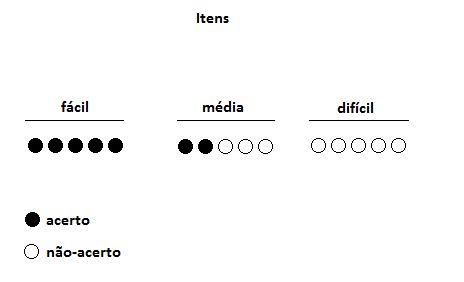
\includegraphics[width=0.5\linewidth]{img/coerente}}\\
		fonte: Autor
		\label{fig:coerente}
	\end{figure}
	\paragraph{}
	    Este padrão é mais corrente, pois o indivíduo acertou os itens fáceis e errou os mais difíceis.
	\begin{figure}[!h]
		\centering
		\caption{padrão incoerente}
		\fbox{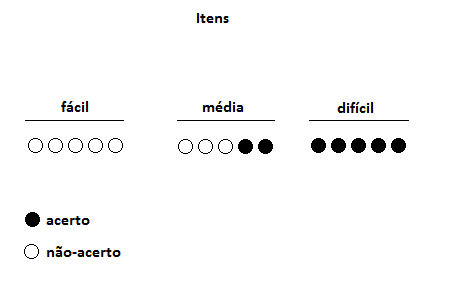
\includegraphics[width=0.5\linewidth]{img/incoerente}}\\
		fonte: Autor
		\label{fig:incoerente}
	\end{figure}
	\paragraph{}
	    Porém, os casos mais comuns Segundo os da Figura(\ref{fig:coerenciax}) no qual o individuo responde corretamente itens acerta itens difíceis ocasionalmente e erra itens fáceis ocasionalmente.
	\begin{figure}[!h]
		\centering
		\caption{padrão mais provável}
		\fbox{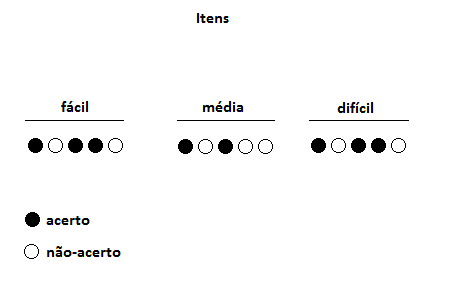
\includegraphics[width=0.5\linewidth]{img/coerenciax}}\\
		fonte: Autor
		\label{fig:coerenciax}
	\end{figure}
	\paragraph{}
	    Entretanto a TRI ao detectar um padrão incoerente como na figura  \ref{fig:incoerente} pode fazer uma analise, julga-se que o individuo que responde corretamente os itens difíceis e responde de forma errada os itens fáceis terá uma nota menor.
	\section{Análise do software EIRT}
	\subsection{Introdução}
	\paragraph{}
	    %https://sourceforge.net/projects/libirt/files/eirt/
    	Com o  crescimento e divulgação da TRI e o avanço computacional deram a TRI instrumentos para cálculos mais complexos, visto que foram implementados softwares para cálculo dos parâmetros e habilidades, como o BILOG e o BILOG-MG. Há ainda o software EIRT, utilizado neste trabalho, um software integrado ao \textit{Microsoft Excel}. O EIRT é uma biblioteca de funções para estimar items e habilidades usando as respostas de indivíduos a um teste/questionário. Os modelos da TRI suportados são os modelos dicotômico e politômicos logísticos de 1,2 e 3 parâmetros, para matriz de respostas pode-se inserir 0/1 ou alternativas dos respondentes, ou uma mistura das duas formas anteriores. Também permite analise de estatísticas referentes a TCT, estimação dos parâmetros do Itens,  dos traços latentes,plotar das curvas características(CCI) de cada item. E para estimação conjunta dos parâmetros e habilidades este software utiliza o EAP(\textit{expected a posteriori}), que o mesmo método empregado pelo INEP nas estimações das notas dos estudantes.
	\par
    	Em seu livro \textcite{Dalton}, apresenta-se os métodos de estimação mais utilizados quando todos os parâmetros dos itens de uma única prova devem ser estimados. No entanto, esta é apenas uma das possíveis situações que na prática iremos encontrar. A seguir, listaremos os 6 casos possíveis, quanto ao número de grupos e de tipos de prova envolvidos.
    \paragraph{}
	\begin{enumerate}
		\item Um único grupo fazendo uma única prova. 
		\item Um único grupo, dividido em dois subgrupos, fazendo duas provas, totalmente distintas (nenhum item comum). 
		\item Um único grupo, dividido em dois subgrupos, fazendo duas provas, apenas parcialmente distintas, ou seja, com alguns itens comuns. 
		\item Dois grupos fazendo uma única prova. 
		\item Dois grupos fazendo duas provas, totalmente distintas (nenhum item comum). 
		\item Dois grupos fazendo duas provas, apenas parcialmente distintas, ou seja, com alguns itens comuns.
	\end{enumerate} 
	\paragraph{}
	    Note que para simplificar, listamos os casos acima utilizando apenas duas provas e duas populações, mas as situações envolvendo um número maior de provas e/ou de populações são análogas.
	\par
    	A análise será feita para para o primeiro caso em que único grupo fazendo uma única prova.A análise será feita a partir de \textit{script}(Anexo  A) feio na linguagem R. R é um software de desenvolvimento para computação estatística e gráfica.
    	Na pratica o \textit{script} executará as seguintes tarefas.
    \subsection{Procedimento}
	\begin{enumerate}
		\item[1 - ] Escolher distribuições para os parâmetros dos itens;
		\item[2 - ] Selecionar 20 alunos(hipotéticos) para responderem os itens;
		\item[3 - ] Para cada aluno escolhe-se uma habilidade;
		\item[4 - ] Fazer uma matriz de respostas dicotomizadas, $1$ se o aluno acertou o item ou $0$ se o mesmo não acertou;
		\item[5 - ] Para cada item escolhe-se um número aleatório entre 0 e 1, se a probabilidade do aluno responder o item for menor que este número então o aluno acerta caso contrário o aluno erra.
	\end{enumerate}
	\paragraph{}
	    Entende-se por matriz de respostas ver tabela(\ref{tab:mat_resposta}), as respostas dos alunos hipotéticos dispostos em forma de tabela de modo que as linhas representem cada aluno e as colunas representem os itens.
	\paragraph{}
	    \begin{table}[!h]
	        \centering
	        \caption{Matriz de resposta}
	        \begin{tabular}{|c|c|c|c|c|c|}
	           \hline
	              & item 1 & item 2 & item 3 & ... & item i\\
	           \hline
	           \hline
	             aluno 1 & $U_{11}$ & $U_{12}$ & $U_{13}$ & ... & $U_{1i}$\\
	           \hline
	             aluno 2 & $U_{21}$& $U_{22}$ & $U_{23}$ & ... & $U_{2i}$\\
	           \hline
	             aluno 3 & $U_{31}$ & $U_{32}$ & $U_{33}$ & ... & $U_{3i}$\\
	           \hline
	             aluno 4 & $U_{41}$ & $U_{42}$ & $U_{43}$ & ... & $U_{4i}$\\
	           \hline
	             aluno 5 & $U_{51}$ & $U_{52}$ & $U_{53}$ & ... & $U_{5i}$\\
	           \hline
	               ...   & ... & ... & ... & ... & ...\\
	           \hline
	             aluno N & $U_{j1}$ & $U_{j2}$ & $U_{j3}$ & ... & $U_{ij}$\\
	           \hline
	        \end{tabular}
	        \label{tab:mat_resposta}
	    \end{table}
	   
	    \newpage
	     As distribuições paras os parâmetros será os seguintes://
	 
	    \begin{enumerate}
	        \item  Para o parâmetro a do discriminação, uma distribuição normal com média 0 e desvio padrão 1.
	        \item 	Como os parâmetros de dificuldade estão na mesma escala de habilidade, em geral, supõem-se que cada $b_is$ tem distribuição Normal,  uma distribuição normal com média 0 e desvio padrão 1.
	        \item 	Para o parâmetro de acerto casual, uma distribuição normal com média 0,2 e desvio padrão 0.01(para um item no qual é permitido chutar o valor esperado para seu parâmetro de acerto casual é próximo a 1/N onde N é a quantidade de alternativas. Para o caso de dos itens aqui testados teram 5 alternativas).
	        \item depois o \textit{script} fará uma matriz de zeros e uns.\\
	    \end{enumerate}
    Os dados gerados pelo \textit{script} estão aqui dispostos, e para uma melhor visualização apresentados através de suas distribuições de frequências.\
	O histograma da figura(\ref{fig:a}) mostra as distribuições para o parâmetro de discriminação de 50 itens.\\
	\begin{figure}[!h]
		\centering
		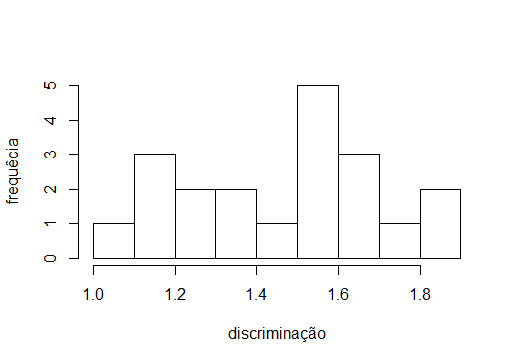
\includegraphics[width=0.6\linewidth]{img/a}
		\caption{}
		\label{fig:a}
	\end{figure}
	
	\newpage
	
	O histograma da figura(\ref{fig:b}) mostra as distribuições para o parâmetro de dificuldade dos 20 itens
	
	\begin{figure}[!h]
		\centering
		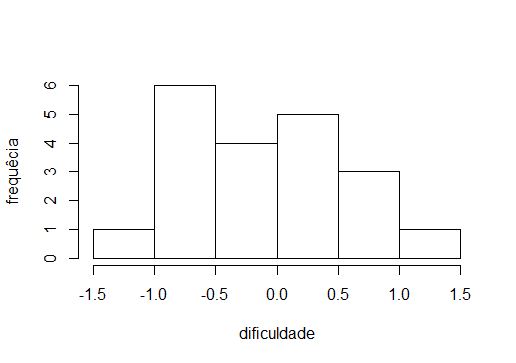
\includegraphics[width=0.6\linewidth]{img/b}
		\caption{}
		\label{fig:b}
	\end{figure}
	
	O histograma da figura(\ref{fig:c})  mostra as distribuições para o parâmetro de acerto ao acaso dos 20 itens.
	\begin{figure}[!h]
		\centering
		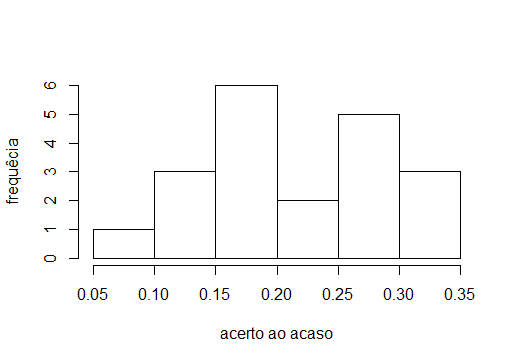
\includegraphics[width=0.6\linewidth]{img/c}
		\caption{}
		\label{fig:c}
	\end{figure}
	\newpage
	O histograma da figura(\ref{fig:hab}) mostra as distribuições para as habilidades dos 20 respondentes.
	\begin{figure} [!h]
		\centering
		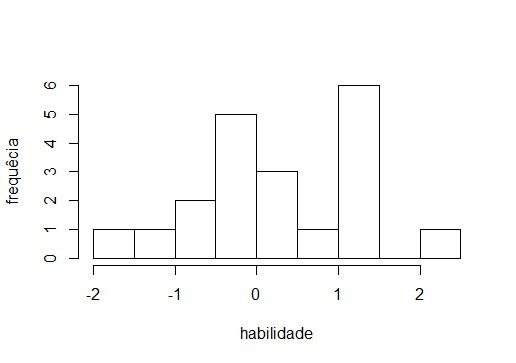
\includegraphics[width=0.6\linewidth]{img/hab}
		\caption{}
		\label{fig:hab}
	\end{figure}
	    A figura(\ref{fig:zeros}) Representa a matriz de zeros e uns, no qual as linhas representam os respondentes e as colunas representam os itens, o valor zero representa que o item foi respondido errado, e um(1) representa que o item foi respondido corretamente. A matriz para 20 respondentes dos 20 alunos(hipotéticos).
    \paragraph{}
		\begin{figure}[!h]
		\caption{Matriz de respostas teste 1}
		\centering
		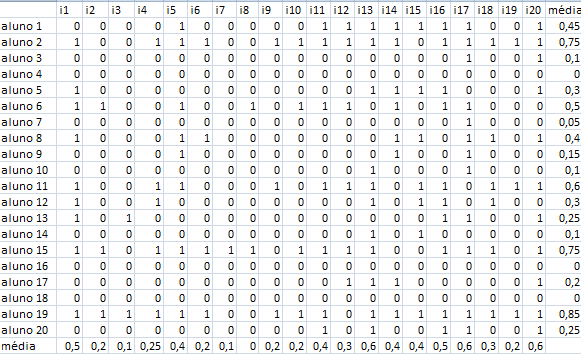
\includegraphics[width=0.6\linewidth]{img/zeros}
		\label{fig:zeros}
	\end{figure}
    importamos estes dados para o \textit{Excel} e utilizamos o software iRTE\\
	Esta imagem mostra curva de todos os itens\\
	\paragraph{}
	\begin{figure}
	    \centering
	    \caption{Todas as CCi}
	    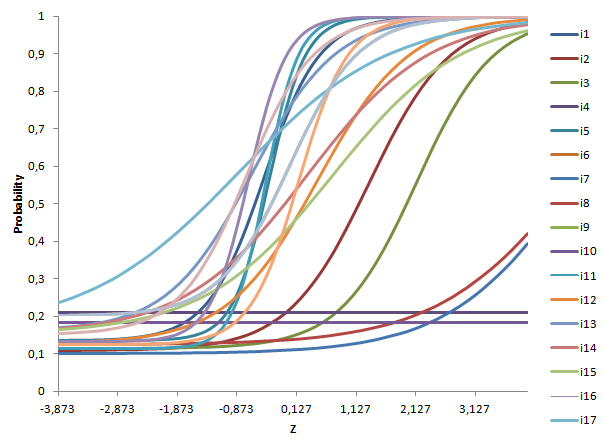
\includegraphics[width=0.5\linewidth]{img/all_cci}
	    \label{fig:all_cci}
	\end{figure}
	    
	para o teste um alguns itens não convergiram:
	i4,i5,i6,i7,i9,i10,i11 e i19
    Estes itens não convergiram,  citado por \textcite{Gleiber}\paragraph{}
   
			\newdimen\mylength
			\mylength = \linewidth
			\addtolength{\mylength}{-4.7cm}
			\hspace{4cm}\begin{minipage}{\mylength}
			    \linespread{1}
				\small{[...] tenta-se manipular os parâmetros do item, produzindo uma curva teórica que mais se aproxime da empírica. O processo de estimação dos parâmetros se encerra quando os valores estimados convergirem, ou seja, quando a partir de n interações não se consegue produzir mais melhorias na reprodução dos dados empíricos por meio das variações nos valores dos parâmetros dos itens. (Wright e Stone, 2004; Baker, 2001; Muñiz, 1990) apud \cite{Gleiber}}
				
			\end{minipage}
		Este fato é facilmente notado através da figura(\ref{fig:all_cci}), o item 1(i4) não se adaptou aos dados, ou seja, a cci do item 1 não se adaptou a uma curva logística.
   \paragraph{}
   
   \begin{table}[!h]
       \centering
       \begin{tabular}{c|c|c|c}
            \hline
            Item &	Slope (a) &	Threshold (b)&	Asymptote (c)\\
            \hline
            \hline
            i1 &	2,126 &	-0,432 & 0,135 \\
            \hline
            i2 &	1,473 &	1,335 &	0,109 \\
            \hline
            i3 &	1,557 &	2,135 &	0,113 \\
            \hline
            i4 &	0,879 &	12,361 &	0,211 \\
            \hline
            i5 &	3,297 &	-0,334 &	0,136 \\
            \hline
            i6 &	0,884 &	19,457 & 0,184 \\
            \hline
            i7 &	0,949 &	4,770 &	0,102 \\
            \hline
            i8 &	0,868 &	4,784 &	0,126 \\
            \hline
            i9 &	1,702 &	0,000 &	0,200 \\ 
            \hline
            i10 &	0,884 &	18,416 &	0,184 \\
            \hline
            i11 &	3,693 &	-0,396 & 0,115 \\
            \hline
            i12 &	1,313 &	0,477 &	0,128 \\
            \hline
            i13 &	1,424 &	-0,628 &	0,163 \\
            \hline
            i14 &	0,974 &	0,305 & 0,154 \\
            \hline
            i15 &	0,927 &	0,736 &	0,155 \\
            \hline
            i16 &	3,140 &	-0,684 &	0,132 \\
            \hline
            i17 &	0,782 &	-0,856 &	0,166 \\
            \hline
            i18 &	2,444 &	0,160 &	0,126 \\
            \hline
            i19 &	1,702 &	0,000 &	0,200 \\
            \hline
            i20 &	1,775 &	-0,718 &	0,152 \\
            \hline
       \end{tabular}
       \caption{Caption}
       \label{tab:my_label}
   \end{table}
   
    \begin{table}[!h]
        \centering
        \begin{tabular}{c|c|c|c}
            \hline
            Subject  &	Z	&	Subject	Z\\
            \hline
            \hline
            aluno 1  &	-0,047	&	aluno 11 &	0,750 \\
            \hline
            aluno 2  &	0,918	&	aluno 12 &	-0,784 \\
            \hline
            aluno 3  &	-1,432	&	aluno 13 &	-0,844 \\
            \hline
            aluno 4  &	-1,839	&	aluno 14 &	-1,522 \\
            \hline
            aluno 5  &	-0,633	&	aluno 15 &	0,437 \\
            \hline
            aluno 6  &	-0,142	&	aluno 16 &	-1,839 \\
            \hline
            aluno 7  &	-1,676	&	aluno 17 &	-1,140 \\
            \hline
            aluno 8  &	-0,604	&	aluno 18 &	-1,839 \\
            \hline
            aluno 9  &	-1,403	&	aluno 19 &	1,419 \\
            \hline
            aluno 10 &	-1,471	&	aluno 20 &	-0,601 \\
            \hline
        \end{tabular}
        \caption{Caption}
        \label{tab:my_label}
    \end{table}
	    
	\paragraph{}
	    Para referência de quais itens são os mais adequados para serem usados em testes Baker( 2001 ) Classifica o parâmetro a da seguinte forma: \\
	\begin{table}[!h]
	    \centering
	    \caption{alguma coisa}
    	\begin{tabular}{|c|c|}
    	    \hline
    	    Muito baixa & de 0,01 a 0,34\\
    	    \hline
    	    Baixa & 0,35 a 0,64\\
    	    \hline
    	    moderada & de 0,64 a 1,34\\
    	    \hline
    	    alta & de 1,35 a 1,69\\
    	    \hline
    	    muito alta & 1,70 \\
    	    \hline
    	\end{tabular}
	\end{table}
	

    \newpage
